\section{Sequenzdiagramme}

Im Folgenden werden zwei der wichtigsten Abläufe des Programms anhand jeweils eines Sequenzdiagramms dargestellt.
Dabei handelt es sich um das Starten und den Ablauf einer Simulation.

\begin{figure}[H]
{\centering 
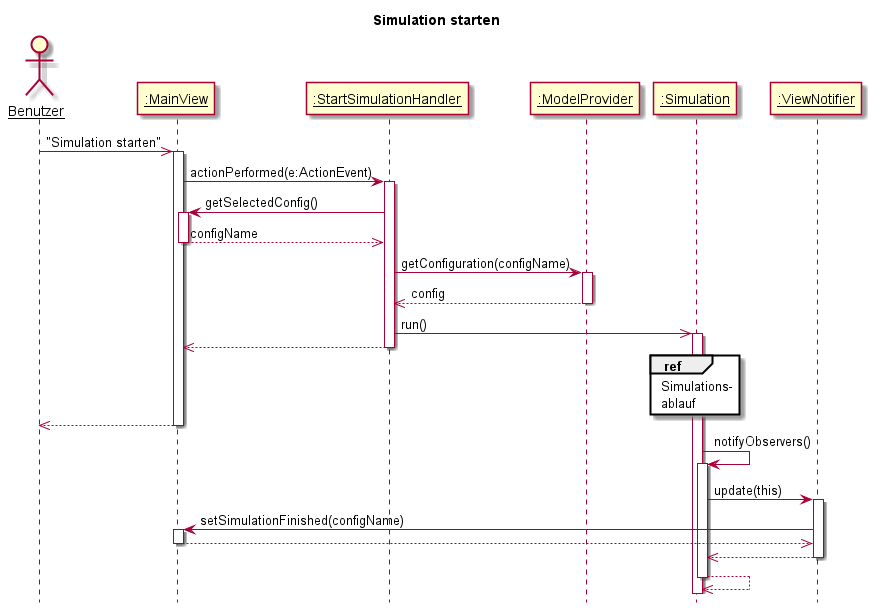
\includegraphics[width=1.0\textwidth]{sequenz_simulationstarten_mitobs}}
\bigskip
\end{figure}

Ausgangspunkt der Sequenz "Simulation starten" ist das Drücken des entsprechenden Buttons im Hauptfenster. Zuvor hat der Benutzer die gewünschte Konfiguration oder Mehrfachkonfiguration ausgewählt.
Im Anschluss unternimmt der StartSimulationHandler die für den Start der Simulation nötigen Vorbereitungen und führt sie schließlich mit run() aus.
Hier setzt die Sequenz "Simulationsablauf" an (s.u.).
Während dem Ablauf der Simulation wird ihr Status durch den ViewNotifier überwacht. Stellt dieser fest, dass die Simulation abgeschlossen ist, benachrichtigt er das Hauptfenster, was die Sequenz beschließt.


\begin{figure}[H]
{\centering 
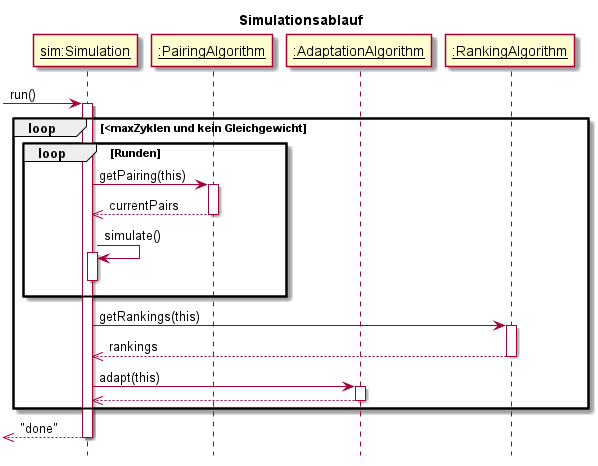
\includegraphics[width=1.0\textwidth]{sequenz_simulation}}
\bigskip
\end{figure}


Die Sequenz "Simulationsablauf" zeigt den eigentlichen Ablauf der Simulation. Dieser besteht im Wesentlichen aus zwei verschachtelten Schleifen. Zum Ende eines jeden Zyklus wird die Simulation auf ein Gleichgewicht überprüft, was ein Abbruchkriterium der äußeren Schleife darstellt.
Die Spiele werden durch simulate() auf der Simulation selbst ausgeführt, wohingegen Manipulationen, die den Datensatz der Simulation betreffen, durch den entsprechenden Algorithmus vorgenommen werden.





